\chapter{An Approach to Support Understanding of Data Leakage in E-Mail Headers}\label{chap:des}

\section{Overview}

In order to satisfy the aims of this project, and building on the presented
objectives, this chapter discusses the requirements of the software intended to
analyse e-mails and the design of the program and its specifications.

\section{Program Specification}

The software should automatically extract information from e-mail headers and
analyse its results to display the personal information contained within an
e-mail's header, as well as information about the software configurations that
may be found on a user's computer, or the servers used to send their e-mail.

The program would be expected to satisfy the following minimal requirements in
order for it to be considered successful: 

\begin{description} 
	
\item [{Accuracy}] --- any information produced by the parser should be
	reflective of the input e-mail

\item [{Representation}] --- the produced visualisation should be intuitive to
	read: each element should be presented separately from the others, and
	clearly labelled.

\item [{Portability}] --- the visual output produced by the program should be
	available to the user in a variety of formats.

\item [{Interactivity}] --- the program should produce sensible warnings when
	an e-mail that is not possible to parse has been entered.

\end{description}

\section{Program Overview}

The program is split up into three main stages: textual analysis and parsing;
header contents analysis, and visualisation, as shown in Figure~\ref{fig:con}.
The relevant data is often stored in a central \texttt{MainWindow} class,
rather than passed as a parameter, as the composition would indicate, allowing
clear references to be maintained.

The  analysis is implemented as a series of stages, firstly, the e-mail header
is parsed, to extract important information to a predefined set of Java objects.
This is followed by the analysis phase, where the resultant data is passed to a
set of analyser modules, each running separately.  Finally, this information is
presented to the user.  After discussing an overview of each module, this chapter 
presents each of these stages in detail.

\begin{figure}
	\centering
\resizebox{0.9\textwidth}{!}{
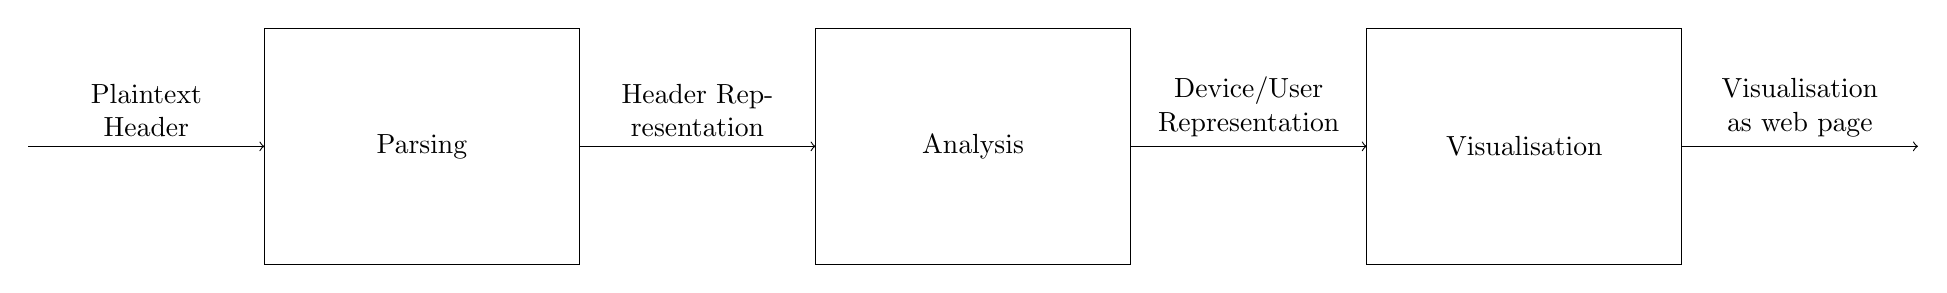
\begin{tikzpicture}
	\draw [->] (-3,1.5) -- (0,1.5) node [above, text width=2.5cm, align=center, midway] { Plaintext Header };
	\draw (0,0) rectangle node {Parsing} (4,3);
	\draw [->] (4,1.5) -- (7,1.5) node [above, text width=2.5cm, align=center, midway] { Header Representation };
	\draw (7,0) rectangle node {Analysis} (11,3);
	\draw [->] (11,1.5) -- (14,1.5) node [above, text width=2.5cm, align=center, midway] { Device/User Representation };
	\draw (14,0) rectangle node {Visualisation} (18,3);
	\draw [->] (18,1.5) -- (21,1.5) node [above, text width=2.5cm, align=center, midway] { Visualisation as web page };
\end{tikzpicture}}
\caption{Simplified Control Flow of Application}
\label{fig:con}
\end{figure}

\subsection{Parsing}

This module receives the plain-text of the e-mail as an input, splitting it
into two sections, fields with the ``Received'' tag, and all other fields.
These are then parsed separately.  The other fields are easier to parse, as
they can be loaded into a hash-map, split by the colon.  The trace fields
require a more complex parsing strategy, fully described in
Section~\ref{sec:par}.  This information is then extracted to more abstract
Java objects, allowing the relevant information to be queried on a
device-by-device basis, rather than constantly referring back to the source
text.

\subsection{Analysis}

The analysis of the e-mail headers is handled independently by a number of
small classes, each running asynchronously.  The decision was made to structure
the program in such a way that concurrent operation was possible in order to
prevent blocking operations from limiting the progress of other operations.
This also required care to ensure the separation between the model of the
header and the model of the available information was maintained, as no
guarantees could be placed on which thread was modifying data.

It is in this part of the program that the automated discovery of
vulnerabilities takes place.  An example software configuration string is
\texttt{cpe:/a:cloudbees:jenkins:2.2}, so it is necessary to attempt to convert
found software information.  For example, \texttt{Apple Mail} would become
\texttt{apple:mail} and a search would be performed over the database for
configurations containing that string.


\subsection{Visualisation}

Once the header has been analysed, it is then necessary to present the
information that has been found in a useful and informative manner. Firstly,
the information about the individual sender, such as their name, organisation,
software and usernames, should be presented (where it exists).  The information
about the servers that the e-mail has passed through should then be detailed, 
their address, location and software, as well as relevant vulnerabilities.

Once this has been listed, information about the scores of the vulnerabilities
for each piece of found software, and a listing of the available
vulnerabilities should be made.  By providing a visualisation of the
distribution of the scores assigned to each piece of software conclusions can 
be drawn about the expected severity of future vulnerabilities.

\section{Comparisons to Existing Software}

\paragraph{Google and Microsoft Header Analysers} Both of the tools discussed
in Sections~\ref{sec:goo} and~\ref{sec:mic} produced detailed information on
the servers that are being used to send and received messages, with Google's
tool also clearly reporting when its own servers were used to send a message.
The software should mimic this by providing a similar level of detail on the
devices being used to send information, and extend this by looking up
information on the device's owning organisation.  Additionally, a more
exhaustive search of the other fields should be conducted, so more information
about the sender can be provided than the immediately available details such as
time, sender's e-mail and recipient.

\paragraph{MITRE CVE Lookup and Norton Vulnerability Protection} The tools
discussed in Sections~\ref{sec:mit} and~\ref{sec:nor} are both targeted at very
different demographics.  The MITRE CVE Lookup is designed for IT professionals
and system administrators wishing to gather more information about specific
vulnerabilities and software, requiring knowledge of the software present on a
network or device.  The information presented is also not structured or sorted
in a clear fashion.

Norton's tool, on the other hand, is focused on individual users who administer
their own systems.  The information is presented in such a way as to warn them
as to which software needs updating or patching against a vulnerability, but
provides few details on the nature of the vulnerabilities.

The tool that is described in this report ought to be able to bridge the gap
between these two tools, providing a useful and relevant list of
vulnerabilities, without overloading the information provided, or requiring
complex search terms to be crafted. 

\section{Typical Use}

On starting the application, the user will provide an e-mail that they wish
to have analysed.  This will then be parsed, and some relevant information
presented in a table.

Lastly, an option is available to view the information about security
vulnerabilities in a separate webpage, forming the main output of the
program.

The resultant webpage will be structured as in Table~\ref{tab:format}.  It
will then be possible for the user to click on the representations of the
devices to find out more information.  It will also be possible to search
within the vulnerability list to find more information, as well as filter by
impact and availability details.

  \begin{table}[] \centering \begin{tabular}{@{}clllll@{}} \toprule
    \multicolumn{6}{c}{Email Header Information}                                                                                                                                                                                                                                      \\
    \midrule \multicolumn{2}{l}{\begin{tabular}[c]{@{}l@{}}Sender Information\\
    (Name, originating domain)\end{tabular}} & \multicolumn{2}{l}{Sender
    Software} & \multicolumn{2}{l}{\begin{tabular}[c]{@{}l@{}}Sender Usernames\\
    (Presented as a list with likely organisation)\end{tabular}} \\
    \midrule
    \multicolumn{6}{c}{Graphical representation of devices used to deliver the
    e-mail}                                                                                                                                                                                                \\
    \midrule
    \multicolumn{6}{c}{List of derived information including found software and
    similar information}                                                                                                                                                                                  \\
    \midrule
    \multicolumn{6}{c}{Histograms for vulnerability scores, separated by
    product}                                                  \\
    \midrule
    \multicolumn{6}{c}{Table of discovered CVEs that can be searched and filtered}                                                                                                                                                                                                            \\
    \bottomrule \end{tabular} \caption{Format of presented data found in e-mail
    header}\label{tab:format} \end{table}

